\documentclass[a4paper,12pt]{article}
\usepackage[utf8]{vietnam}
\usepackage[utf8]{inputenc}
\usepackage{amsmath}
\usepackage{amsfonts}
\usepackage{array}
\usepackage{amssymb}
\usepackage{graphicx}
\usepackage[margin=1in]{geometry}
\usepackage{longtable}
\usepackage{xspace}
\usepackage{booktabs} % For formal tables
\usepackage{makecell} % Allows for multi-line cells
\usepackage{xcolor} % For cell coloring
\usepackage{graphicx} % For scaling tables
% \usepackage{caption}
\usepackage{booktabs} % For formal tables
\usepackage{tabularx} % For adjustable-width columns
\usepackage{makecell} % Allows for multi-line cells
\usepackage{xcolor} % For cell coloring
\usepackage{graphicx} % For scaling tables
\usepackage[margin=1in]{geometry} % Adjust page margins if necessary
\usepackage[font=small]{caption}
\usepackage{booktabs}
\usepackage[unicode]{hyperref}
\usepackage{titlesec} 
\usepackage{scrextend}
\usepackage{enumerate}
\usepackage{url}
\usepackage{tikz}
\usepackage{float}
\usepackage{afterpage}
\usepackage{multirow}
\usepackage{sectsty}
\usepackage{tocloft,calc}
\usepackage{listings}
\usepackage{makecell}
\usepackage[sort&compress]{natbib}
\usetikzlibrary{calc}
\usepackage{algorithm}
\usepackage{bookmark}
\usepackage{algpseudocode}
\usepackage{subcaption}
% \usepackage{minted}
% \usepackage[perpage]{footmisc}
\usepackage[flushleft]{threeparttable}
% \usepackage{subcaption}
\usepackage{perpage} %the perpage package
\MakePerPage{footnote} %the perpage package command
% \usepackage[ruled,vlined]{algorithm2e}
\PassOptionsToPackage{table}{xcolor}
\newcommand{\Emptyset}{\text{\o}}
\usepackage{lmodern}
\usepackage{mathtools}
\usepackage{graphicx} % Required for inserting images
\usepackage{subcaption}
\begin{document}

\thispagestyle{empty}

\begin{tikzpicture}[remember picture, overlay]
  \draw[line width = 2pt] ($(current page.north west) + (0.5in,-0.5in)$) rectangle ($(current page.south east) + (-0.5in,0.5in)$);
\end{tikzpicture}

\begin{center}
\changefontsizes{14pt}

	\textbf{ĐẠI HỌC QUỐC GIA HÀ NỘI\\TRƯỜNG ĐẠI HỌC CÔNG NGHỆ}\\[1cm]
	
\includegraphics[width=0.2\linewidth]{images/uet.jpg}\\[0.3cm]
        \textbf{BÁO CÁO BÀI TẬP LỚN XỬ LÝ ẢNH INT3404E 20}
        \\
        \textbf{NĂM HỌC 2023 – 2024}
	\\[2cm]
	\large{\textbf{Tên báo cáo:}} \\
	\large{\textbf{OBJECT LOCALIZATION FOR SINO NOM'S CHARACTER WITH YOLO FRAMEWORK}}
	\\[2.6cm]
        \begin{tabular}{l l}
    
            Nhóm 2: &{Tăng Vĩnh Hà - K67-CA-CLC2} \\
            &{Lê Thị Hải Anh - K67-CA-CLC2} \\
            &{Vũ Nguyệt Hằng - K67-CA-CLC2} \\ 
            &{Lê Xuân Hùng - K67-CA-CLC2} \\
            \\[0.25cm]
            
            Giáo viên hướng dẫn: &{GS. Lê Thanh Hà}\\
            &{ThS. Nguyễn Công Thương}\\
            
        \end{tabular}
	% \normalsize{\textbf{BÁO CÁO NGHIÊN CỨU KHOA HỌC
	% 	\\[2mm]
	% Ngành: Khoa học máy tính}}

	\vfill
	\textbf{HÀ NỘI - 2024}
	\vspace{10mm}
\end{center}
\clearpage

\section{Tóm tắt}
\begin{figure}[ht]
    \centering
    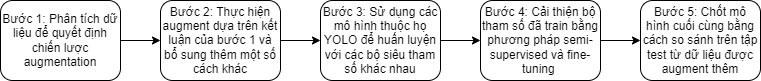
\includegraphics[width=0.5\linewidth]{images/Pipeline.png}
    \caption{Pipeline cơ bản của nhóm}
\end{figure}

\section{Phương pháp}
\subsection{Phân tích dữ liệu}

Trước khi train model, nhóm đã thực hiện phân tích qua về dữ liệu của label trong tập train.
\\
Ở đây, có 3 hướng chính để tiếp cận dữ liệu như sau:
\begin{itemize}
    \item Hướng tiếp cận 1: Vẽ các biểu đồ histogram từng aspect (tọa độ x, y, chiều dài chiều rộng) của ký tự trên toàn tập ảnh
    \item Hướng tiếp cận 2: Tính 
    \item Hướng tiếp cận 3: Phân loại các ảnh đặc biệt có nguy cơ bị lỗi
\end{itemize}
\subsubsection{Hướng tiếp cận 1: Vẽ các biểu đồ histogram từng aspect}
Ở đây, aspect gồm 4 mục:
\begin{itemize}
    \item Tọa độ x, y của các kí tự (các Bounding Box)
    \item Chỉ số chiều dài, rộng của Bounding Box w, h
\end{itemize}
Đầu tiên, tạo biểu đồ histogram thể hiện sự phân tán của tọa độ x, y của từng kí tự trong tất cả các ảnh 
\\
\begin{figure}[ht]
    \centering
    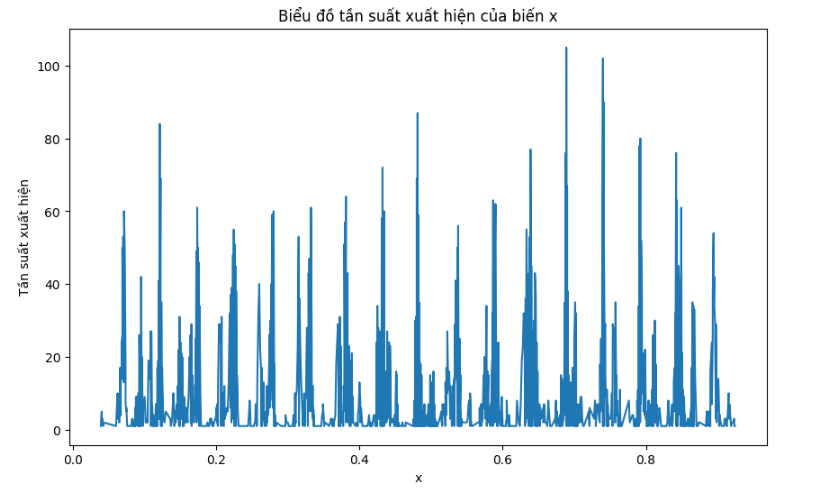
\includegraphics[width=1\linewidth]{images/HistoX_dis_train.png}
    \caption{Phân bố của tọa độ x}
\end{figure}
\begin{figure}[ht]
    \centering
    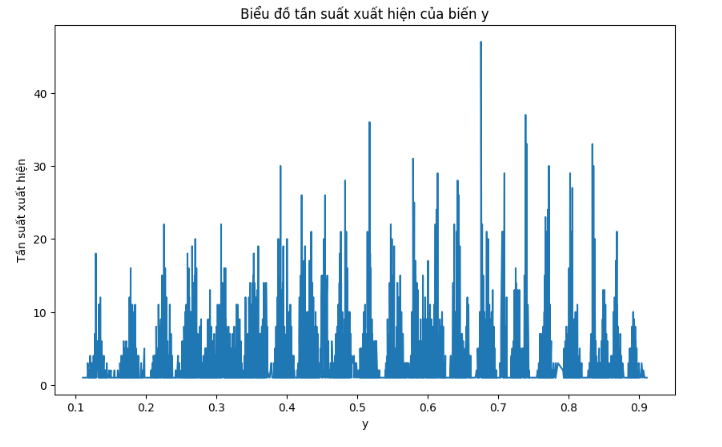
\includegraphics[width=1\linewidth]{images/HistoY_dis_train.png}
    \caption{Phân bố của tọa độ y}
\end{figure}
$\rightarrow$ Các ảnh phân bố cho thấy tọa độ $x$, $y$ của các kí tự phân bố khá đều, nhìn biểu đồ ta thấy tập trung nhiều nhất trong tọa độ $x$ $\in$ $[0.6, 0.7]$; $y$ $\in$ $[0.65, 0.7]$.
\\
$\rightarrow$ Có thể sinh $cropped\_imgs$ của vùng này trên $70$ cái ảnh tập $train$ nhưng phân bố của tọa độ $x$, $y$ trải đều thì không bị coi là tập trung quá nhiều (bất thường).

Tiếp theo, ta quan sát phân bố của chiều dài và chiều rộng của tất cả các Bounding Box
\begin{figure}[ht]
    \centering
    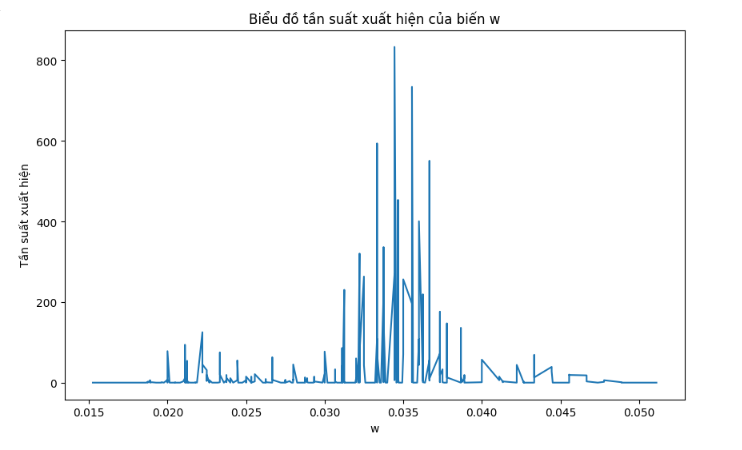
\includegraphics[width=1\linewidth]{images/HistoW_train.png}
    \caption{Phân bố của chiều rộng các BB}
    %\label{fig:enter-label}
\end{figure}
$\rightarrow$ Chiều rộng các Bounding Box phân bố tập trung từ 0.03 đến 0.045.
\\
\begin{figure}[ht]
    \centering
    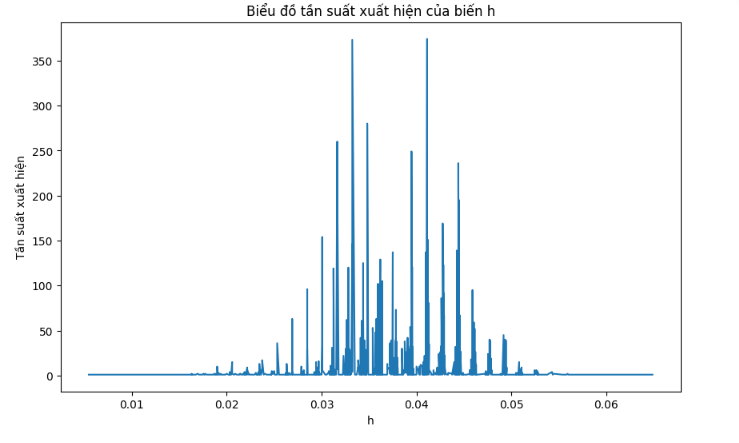
\includegraphics[width=1\linewidth]{images/HistoH_train.png}
    \caption{Phân bố của chiều dài các BB}
    %\label{fig:enter-label}
\end{figure}
$\rightarrow$ Chiều dài các BB từ 0.03 đến 0.04
\subsubsection{Hướng tiếp cận 2: Xét xem variance từng aspect của Bounding Box trong 1 ảnh có bị lệch không}
Phần này t định sort các ảnh có variance cao (độ lệch so với giá trị trung cao). Thế nhưng t nghĩ là variance cao có thể do nhiều yếu tố nữa => hướng này tạm để cuối.
\subsubsection{Hướng tiếp cận 3: Phân loại các ảnh đặc biệt có nguy cơ bị lỗi}
Trong một lần train với số epoch thấp thì vô tình phát hiện được ra là model làm tốt ở các ảnh chữ thưa và làm không tốt ở các ảnh chữ không thưa.
\\
\textbf{Ý tưởng chung}: Ta sẽ xét xem các Bounding Box của ảnh có tập trung quá nhiều vào 1 nửa của ảnh hay không. Nếu có thì khả năng lỗi ở ảnh đó sẽ cao hơn.
Để cụ thể hóa hơn, ta chia ảnh thành 2 nửa (có 2 cách chia: chia theo chiều dọc và chiều ngang) và ta xây dựng 1 ngưỡng rate.
\\
Ở đây, rate là tỉ lệ độ thưa thể hiện nửa ảnh có số kí tự ít hơn rate\% hay không, miền giá trị của rate là [0; 0.5].
\\
Nếu một nửa ảnh có số ký tự nhỏ hơn rate\% của ảnh thì ảnh đó sẽ bị liệt vào danh sách những ảnh có nguy cơ bị lỗi, ta gọi các ảnh này là các ảnh bị lệch.
\\
Danh sách các ảnh bị lệch sẽ tăng khi ta tăng rate lên.
\\
Đôi khi rate cao quá thì điều kiện lọc sẽ bị quá dễ $\rightarrow$ rất nhiều ảnh không đến mức dễ lỗi mà bị lọc là lỗi.
\\
$\rightarrow$ Nhóm thực hiện sinh với các rates là $0.3$ và $0.35$ vì trước đó đã thử với nhiều rate khác nhau thì quan sát được rate từ $0.3 -> 0.35$ cho dữ liệu tin cậy (nhìn nhận qua folder ảnh).
\\
Sau đó, nhóm quyết định sinh ra nhiều bộ dữ liệu với các rate khác nhau vd bộ 1 gồm $original + rate\_0.3$ và bộ $2$ gồm $original + rate\_0.4$ rồi đưa vào train model xem bộ dữ liệu nào tốt hơn. 
\subsubsection{Phân tích distribution của tập val có gì bất thường so với train không}
Nhóm đã vẽ các biểu đồ Histogram (giống Hướng tiếp cận 1 đã nêu) trên tập labels val và không phát hiện bất thường so với tập labels train từ các aspect của Bounding Box.
\subsubsection{Phân tích sự đồng đều kích cỡ của các ảnh}
Quan sát các ảnh trên tập dữ liệu train, kích cỡ các ảnh có khác nhau nhưng chủ yếu có 3 nhóm kích cỡ dựa theo tên của các ảnh (Ví dụ tên ảnh là "nlvnpf-0137-01-001" thì ảnh thuộc nhóm kích cỡ "0137"). Cụ thể hơn 3 nhóm có kích cỡ W x H như sau:
\begin{itemize}
    \item Nhóm 0137: 900 x 608
    \item Nhóm 0140: 750 x 640
    \item Nhóm 0174: 800 x 632
\end{itemize}
Mỗi nhóm có chung chỉ số W còn H giao động quanh số đã nêu ở trên.

\subsection{Tiền xử lý dữ liệu}
%Hằng và Sone ghi vào đây
Trong phần này, nhóm xin trình bày về việc tiền xử lý dữ liệu bằng cách tăng cường dữ liệu (augmentation) cho tập dữ liệu ảnh và nhãn. Việc tăng cường dữ liệu ảnh đã được thực hiện trên dữ liệu ảnh ban đầu ($original$ $data$) và dữ liệu ảnh đặc biệt có nguy cơ bị lỗi theo hướng tiếp cận 3 đã đề cập với $rate=0.3$ và $rate=0.35$.
\subsubsection{Các kĩ thuật augmentation cơ bản}
%Sone viết những cái sau vì Sone đã làm rồi
Nhóm đã sử dụng thư viện $albumentations$ của Python hỗ trợ để thực hiện các kỹ thuật augmentation cơ bản sau đây:
\begin{itemize}
    \item Xoay ảnh theo nhiều góc
    \\Để tạo ra các phiên bản mới của ảnh và nhãn, nhóm đã sử dụng phép xoay ảnh với nhiều góc khác nhau trong đó giới hạn là $15^\circ$. Quá trình này giúp tăng cường dữ liệu bằng cách tạo ra các ảnh có góc nhìn khác nhau, từ đó làm tăng tính đa dạng của tập dữ liệu.
    
    \begin{figure}[H]
        \centering
        \begin{subfigure}{.4\textwidth}
          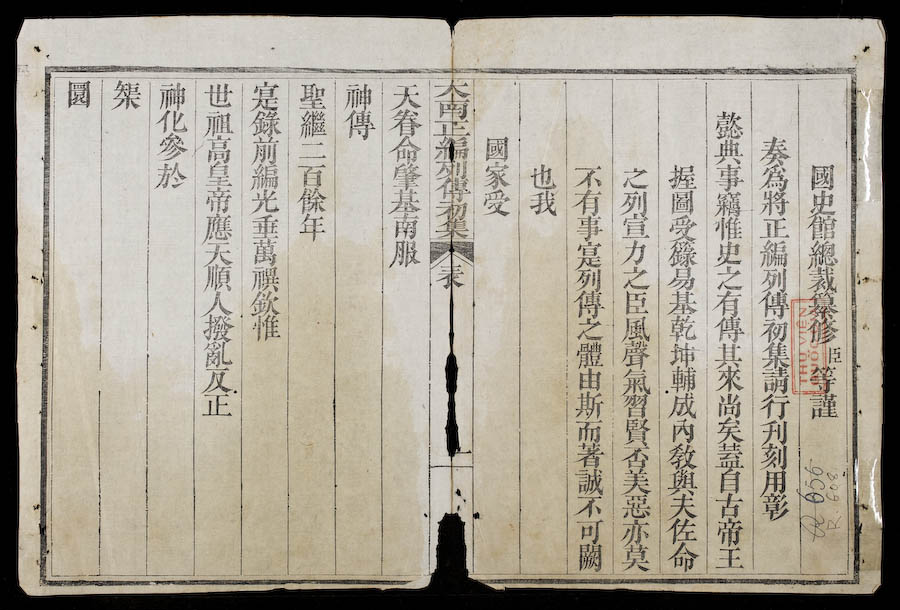
\includegraphics[width=1\linewidth]{images/original_img_1.jpg}
          \caption{Ảnh gốc}
        \end{subfigure}
        \hspace{20mm}
        \begin{subfigure}{.4\textwidth}
          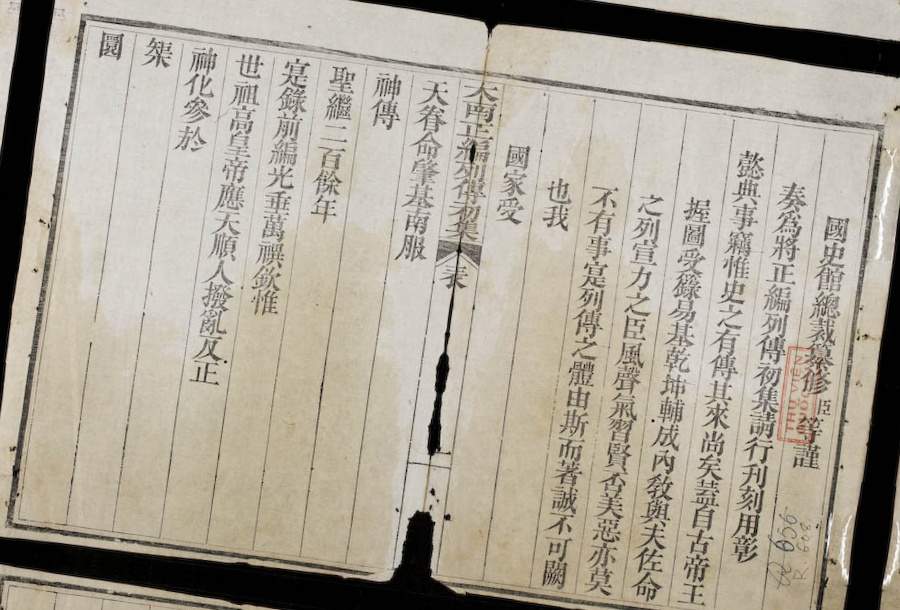
\includegraphics[width=1\linewidth]{images/rotated_img.png}
          \caption{Ảnh sau khi xoay góc}
        \end{subfigure}
        \caption{Kết quả phép xoay ảnh theo góc giới hạn $15^\circ$}
    \end{figure}

    \item Add noise
    %thực hiện lên bộ ảnh mà Hùng quyết định tập trung.
    \\Nhóm đã áp dụng kỹ thuật thêm nhiễu vào ảnh để tạo ra các phiên bản mới với độ nhiễu khác nhau. Việc này giúp tạo ra sự đa dạng trong dữ liệu và làm tăng khả năng tổng quát hóa của mô hình.
    Nhóm sử dụng $2$ loại nhiễu để thêm vào ảnh chỉnh là gaussian noise và multipricate noise
    \begin{figure}[H]
        \centering
        \begin{subfigure}{.4\textwidth}
          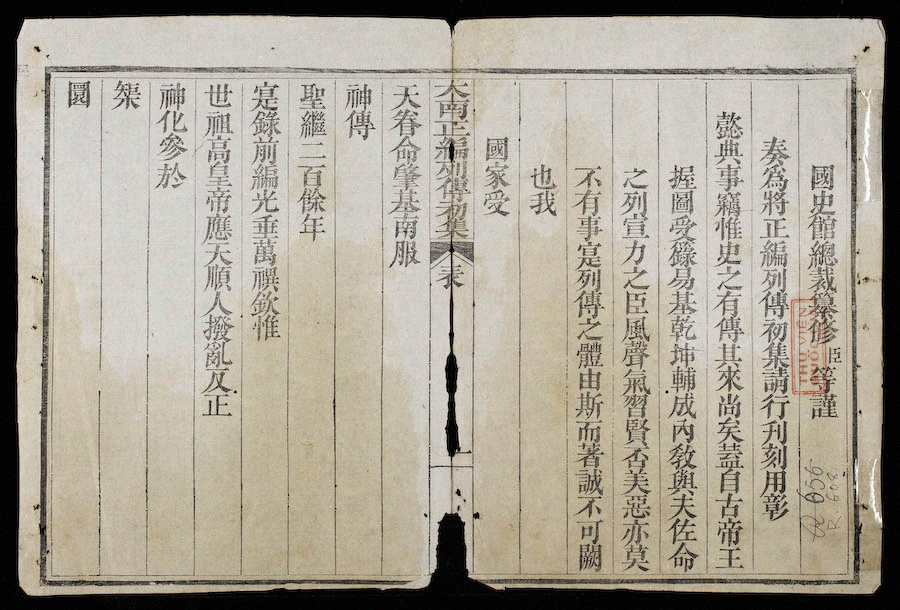
\includegraphics[width=1\linewidth]{images/gaussian_img.png}
          \caption{Ảnh thêm nhiễu gaussian}
        \end{subfigure}
        \hspace{20mm}
        \begin{subfigure}{.4\textwidth}
          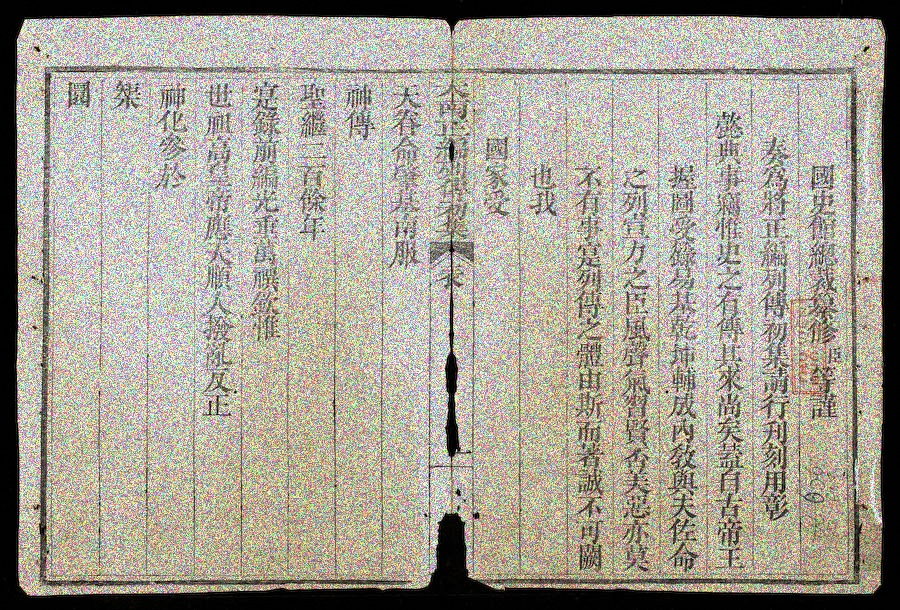
\includegraphics[width=1\linewidth]{images/multipricate_img.png}
          \caption{Ảnh thêm nhiễu multipricate}
        \end{subfigure}
        \caption{Kết quả phép thêm nhiễu}
    \end{figure}
    \item Scale ảnh
    \\Nhóm đã thực hiện phép biến đổi scale ảnh để tạo ra các phiên bản mới có kích thước khác nhau. Điều này giúp tạo ra các ảnh có kích thước và tỷ lệ khác nhau, từ đó tăng cường tính đa dạng của tập dữ liệu.
    \begin{figure}[H]
        \centering
        \begin{subfigure}{.4\textwidth}
          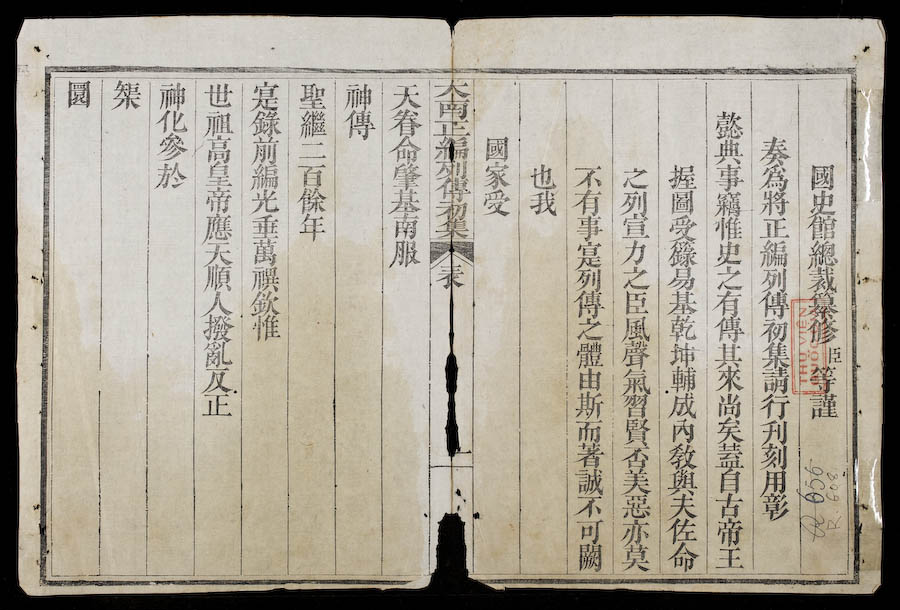
\includegraphics[width=1\linewidth]{images/original_img_1.jpg}
          \caption{Ảnh gốc}
        \end{subfigure}
        \hspace{20mm}
        \begin{subfigure}{.4\textwidth}
          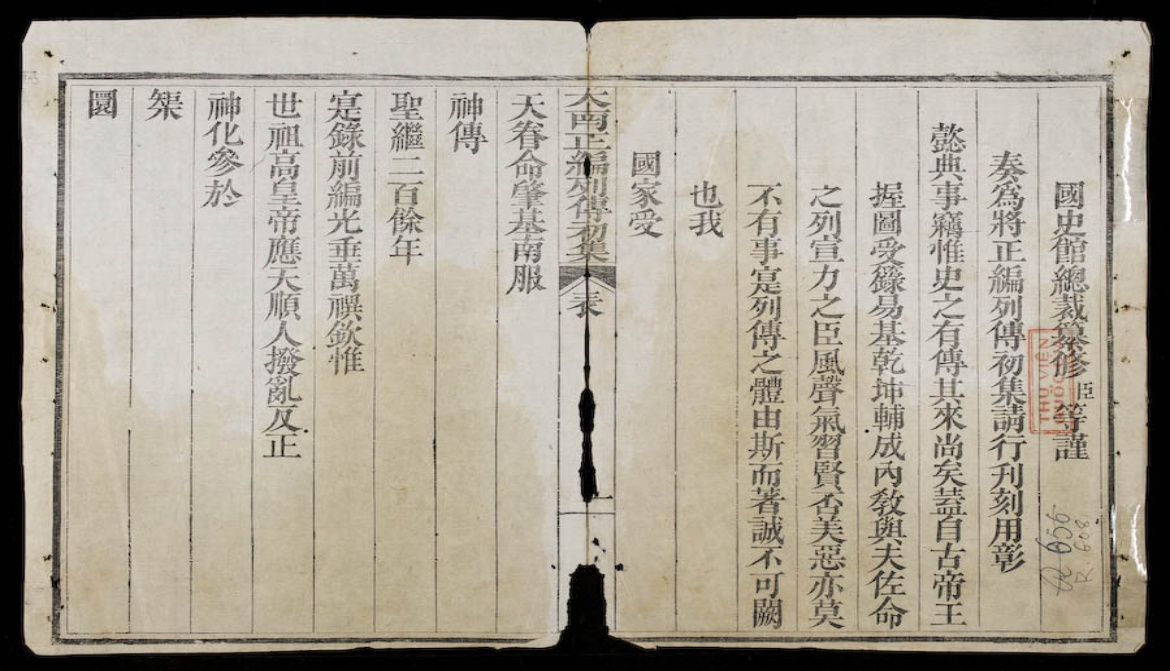
\includegraphics[width=1\linewidth]{images/scaled_img.png}
          \caption{Ảnh sau khi scale}
        \end{subfigure}
        \caption{Kết quả phép scale ảnh}
    \end{figure}
    \item Dịch chuyển ảnh sang trái phải
    \item Crop ảnh chỉ show 1 phần (YOLO có sẵn nên Hà viết)
    \item Các kỹ thuật augmen khác được tích hợp sẵn trong framework YOLOv8 (Hà viết)
\end{itemize}
\subsubsection{Các kĩ thuật augmentation nâng cao}

\begin{itemize}
    \item Kết hợp nhiều kỹ thuật augmentation trong cùng 1 bức ảnh
    \\Nhóm đã kết hợp nhiều kỹ thuật augmentation cơ bản trong cùng một bức ảnh. Trong đó, ngoài $3$ phép biến đổi đã đề cập, nhóm đã kết hợp thêm các phép biến đổi như $Horizontal\_flip$, $Blur$ và $BrightnessContrast$, trong đó mỗi phép biến đổi con được thực hiện với xác suất $p=0.5$
    \begin{figure}[H]
        \centering
        \begin{subfigure}{.4\textwidth}
          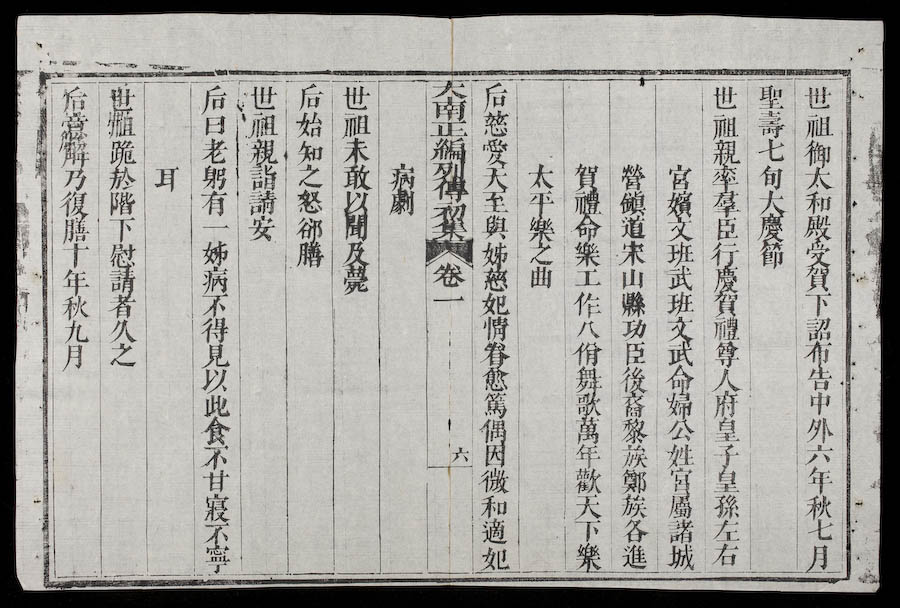
\includegraphics[width=1\linewidth]{images/original_img_2.jpg}
          \caption{Ảnh gốc}
        \end{subfigure}
        \hspace{20mm}
        \begin{subfigure}{.4\textwidth}
          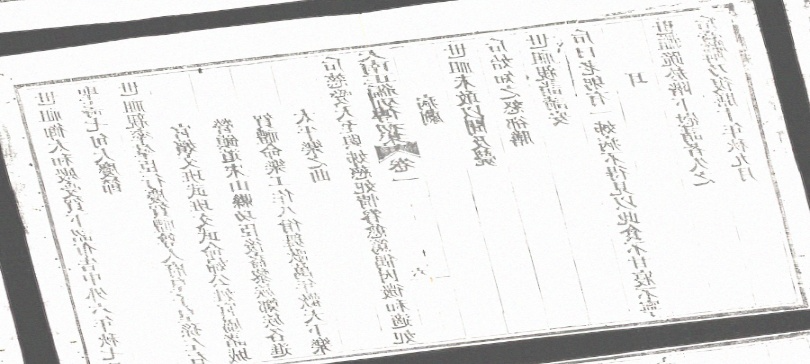
\includegraphics[width=1\linewidth]{images/combined_img.png}
          \caption{Ảnh sau biến đổi với nhiều kỹ thuật}
        \end{subfigure}
        \caption{Kết quả phép biến đổi kết hợp nhiều kỹ thuật}
    \end{figure}
    \item Chuẩn hóa ảnh (không rõ YOLOv8 có làm hay không để Hà tìm hiểu)
\end{itemize}
\subsection{Thuật toán xác định bounding box}
\subsubsection{YOLOv5}
% \begin{itemize}
%     \item 
% \end{itemize}
\paragraph{Tổng quan kiến trúc}
\paragraph{Tổng quan thư viện Ultralytics}
\paragraph{Áp dụng vào bài toán detect chữ Nôm}
\subsubsection{YOLOv8}
\paragraph{Tổng quan kiến trúc}
\paragraph{Áp dụng vào bài toán detect chữ Nôm}
\subsection{Validation}
\section{Kết quả}
\section{Kết luận và thảo luận}
\end{document}
